% Template for PLoS
% Version 3.1 February 2015
%
% To compile to pdf, run:
% latex plos.template
% bibtex plos.template
% latex plos.template
% latex plos.template
% dvipdf plos.template
%
% % % % % % % % % % % % % % % % % % % % % %
%
% -- IMPORTANT NOTE
%
% This template contains comments intended 
% to minimize problems and delays during our production 
% process. Please follow the template instructions
% whenever possible.
%
% % % % % % % % % % % % % % % % % % % % % % % 
%
% Once your paper is accepted for publication, 
% PLEASE REMOVE ALL TRACKED CHANGES in this file and leave only
% the final text of your manuscript.
%
% There are no restrictions on package use within the LaTeX files except that 
% no packages listed in the template may be deleted.
%
% Please do not include colors or graphics in the text.
%
% Please do not create a heading level below \subsection. For 3rd level headings, use \paragraph{}.
%
% % % % % % % % % % % % % % % % % % % % % % %
%
% -- FIGURES AND TABLES
%
% Please include tables/figure captions directly after the paragraph where they are first cited in the text.
%
% DO NOT INCLUDE GRAPHICS IN YOUR MANUSCRIPT
% - Figures should be uploaded separately from your manuscript file. 
% - Figures generated using LaTeX should be extracted and removed from the PDF before submission. 
% - Figures containing multiple panels/subfigures must be combined into one image file before submission.
% For figure citations, please use "Fig." instead of "Figure".
% See http://www.plosone.org/static/figureGuidelines for PLOS figure guidelines.
%
% Tables should be cell-based and may not contain:
% - tabs/spacing/line breaks within cells to alter layout or alignment
% - vertically-merged cells (no tabular environments within tabular environments, do not use \multirow)
% - colors, shading, or graphic objects
% See http://www.plosone.org/static/figureGuidelines#tables for table guidelines.
%
% For tables that exceed the width of the text column, use the adjustwidth environment as illustrated in the example table in text below.
%
% % % % % % % % % % % % % % % % % % % % % % % %
%
% -- EQUATIONS, MATH SYMBOLS, SUBSCRIPTS, AND SUPERSCRIPTS
%
% IMPORTANT
% Below are a few tips to help format your equations and other special characters according to our specifications. For more tips to help reduce the possibility of formatting errors during conversion, please see our LaTeX guidelines at http://www.plosone.org/static/latexGuidelines
%
% Please be sure to include all portions of an equation in the math environment.
%
% Do not include text that is not math in the math environment. For example, CO2 will be CO\textsubscript{2}.
%
% Please add line breaks to long display equations when possible in order to fit size of the column. 
%
% For inline equations, please do not include punctuation (commas, etc) within the math environment unless this is part of the equation.
%
% % % % % % % % % % % % % % % % % % % % % % % % 
%
% Please contact latex@plos.org with any questions.
%
% % % % % % % % % % % % % % % % % % % % % % % %

\documentclass[10pt,letterpaper]{article}
\usepackage[top=0.85in,left=2.75in,footskip=0.75in]{geometry}

% Use adjustwidth environment to exceed column width (see example table in text)
\usepackage{changepage}

% Use Unicode characters when possible
\usepackage[utf8]{inputenc}

% textcomp package and marvosym package for additional characters
\usepackage{textcomp,marvosym}

% fixltx2e package for \textsubscript
\usepackage{fixltx2e}

% amsmath and amssymb packages, useful for mathematical formulas and symbols
\usepackage{amsmath,amssymb}

% cite package, to clean up citations in the main text. Do not remove.
\usepackage{cite}

% Use nameref to cite supporting information files (see Supporting Information section for more info)
\usepackage{nameref,hyperref}

% line numbers
\usepackage[right]{lineno}

% ligatures disabled
\usepackage{microtype}
\DisableLigatures[f]{encoding = *, family = * }

% rotating package for sideways tables
\usepackage{rotating}

% ADDED BY NICK JAGIELLA
\usepackage{color}
\usepackage{grffile}
%\usepackage{minitoc}

% Remove comment for double spacing
%\usepackage{setspace} 
%\doublespacing

% Text layout
\raggedright
\setlength{\parindent}{0.5cm}
\textwidth 5.25in 
\textheight 8.75in

% Bold the 'Figure #' in the caption and separate it from the title/caption with a period
% Captions will be left justified
\usepackage[aboveskip=1pt,labelfont=bf,labelsep=period,justification=raggedright,singlelinecheck=off]{caption}

% Use the PLoS provided BiBTeX style
\bibliographystyle{plos2015}

% Remove brackets from numbering in List of References
\makeatletter
\renewcommand{\@biblabel}[1]{\quad#1.}
\makeatother

\newcommand{\jh}[1]{{\color{red}#1}}

% Leave date blank
\date{}

% Header and Footer with logo
\usepackage{lastpage,fancyhdr,graphicx}
\usepackage{epstopdf}
\pagestyle{myheadings}
\pagestyle{fancy}
\fancyhf{}
\lhead{\includegraphics[width=2.0in]{PLOS-submission.eps}}
\rfoot{\thepage/\pageref{LastPage}}
\renewcommand{\footrule}{\hrule height 2pt \vspace{2mm}}
\fancyheadoffset[L]{2.25in}
\fancyfootoffset[L]{2.25in}
\lfoot{\sf PLOS}

%% Include all macros below

\newcommand{\lorem}{{\bf LOREM}}
\newcommand{\ipsum}{{\bf IPSUM}}

%% END MACROS SECTION


\begin{document}
\vspace*{0.35in}

% Title must be 250 characters or less.
% Please capitalize all terms in the title except conjunctions, prepositions, and articles.
\begin{flushleft}
{\Large
\textbf\newline{Approximate Bayesian Computing for Parameter Inference \\[1ex] in Hybrid Discrete-Continuum Models}
}
\newline
% Insert author names, affiliations and corresponding author email (do not include titles, positions, or degrees).
\\
Nick Jagiella\textsuperscript{1},
Dennis Rickert\textsuperscript{1},
Fabian J. Theis\textsuperscript{1,2},
Jan Hasenauer\textsuperscript{1,2,*}
%Name5 Surname\textsuperscript{2,\ddag},
%Name6 Surname\textsuperscript{2},
%Name7 Surname\textsuperscript{3,*},
%with the Lorem Ipsum Consortium\textsuperscript{\textpilcrow}
\\
\bigskip
\bf{1} Helmholtz Zentrum M\"unchen - German Research Center for Environmental Health, Institute of Computational Biology, 85764 Neuherberg, Germany
\\
\bf{2} Technische Universit\"at M\"unchen, Center for Mathematics, Chair of Mathematical Modeling of Biological Systems, 85748 Garching, Germany
\\
\bigskip

% Insert additional author notes using the symbols described below. Insert symbol callouts after author names as necessary.
% 
% Remove or comment out the author notes below if they aren't used.
%
% Primary Equal Contribution Note
%\Yinyang These authors contributed equally to this work.

% Additional Equal Contribution Note
% Also use this double-dagger symbol for special authorship notes, such as senior authorship.
%\ddag These authors also contributed equally to this work.

% Current address notes
%\textcurrency a Insert current address of first author with an address update
% \textcurrency b Insert current address of second author with an address update
% \textcurrency c Insert current address of third author with an address update

% Deceased author note
%\dag Deceased

% Group/Consortium Author Note
%\textpilcrow Membership list can be found in the Acknowledgments section.

% Use the asterisk to denote corresponding authorship and provide email address in note below.
* jan.hasenauer@helmholtz-muenchen.de

\end{flushleft}

\tableofcontents
%\minitoc

%%%%%%
%%%%%%
%%%%%%
% Please keep the abstract below 300 words
\section*{Abstract}
The accurate description of multi-scale biological process requires sophisticated computational models. A variety of tools for the construction and simulations of such models are available. The inference of the unknown parameters of multi-scale models however remains and open problem. Key challenges are stochasticity and computational complexity of most multi-scale models. In this manuscript we present a parallel Approximate Bayesian Computations (pABC) sequential Monte Carlo (SMC) algorithm for the inference of hybrid discrete-continuum models of biological tissue. The propose pABC~SMC algorithm is tailored for large computing clusters with a queuing systems, and allows for the study of stochastic processes. In a simulation example, we verify that the parameters of hybrid discrete-continuum models of tumor spheroids can be inferred reliably. Accordingly, we use the pABC~SMC algorithm to study tumor spheroid growth in droplets, a model for in vivo tumor spread. Interestingly, we find that 2D and 3D models provide similar parameter estimates. Furthermore, the inference results can be used for experimental planning. These results illustrate the feasibility of data-driven modeling of complex multi-scale processes and the reliability of ABC methods.

% Please keep the Author Summary between 150 and 200 words
% Use first person. PLOS ONE authors please skip this step. 
% Author Summary not valid for PLOS ONE submissions.   
\section*{Author Summary}
To do.

\linenumbers

%%%%%%
%%%%%%
%%%%%%
\section*{Introduction}
%<<<<<<< Updated upstream:plos_template.tex

Systems and computational biology aims at a mechanistic understanding of biological systems. To achieve this, biological processes on a wide range of time and length scales have to be captured~\cite{HunterBor2003}. This established the need for multi-scale models. World-wide interdisciplinary initiatives have been formed to develop multi-scale models and modeling approaches for basic research, diagnosis and therapy~\cite{PhysiomeProject}. Among the most well-known projects are the whole-heart~\cite{HunterBor2003,Nobel2002,Trayanova2011} and the whole-cell modeling initiatives~\cite{TomitaHas1999,KarrSan2012}. Furthermore, software toolboxes such as MCell~\cite{StilesBar2001}, VCell~\cite{SchaffFin1997}, FLAME~\cite{}, Deutsch, ... for the implementation and simulation of multi-scale models have been made available. All this resulted in a tremendous increase of the availability and popularity or multi-scale models. A problem which is however largely unsolved is the parameterization of multi-scale models. To enable truly quantitative predictions, the parameters of multi-scale models have to be inferred from experimental data.

For deterministic multi-scale models obtained by coupling ordinary and partial differential equations (O/PDE) promising successes have be achieved. An integrated physiologically based whole-body model of the glucose-insulin-glucagon regulatory system has been developed and parameterized for individual patients to improve the understanding of type~1 diabetes~\cite{SchallerWil2013}. Similarly, whole-heart models could be used to infer ischemic regions from body surface potential maps to provide early diagnosis of heart infarction~\cite{NielsenLys2013}. These and other applications demonstrated that the automated parameterization of multi-scale model from experiment data is feasible. This is however mostly limited to coupled ODE and PDE models, which are deterministic and allow for efficient gradient-based optimization. The parameterization of computationally demanding stochastic model is unsolved\jh{, as the recent DREAM challenge revealed~\cite{}.}

Biological processes such as gene expression~\cite{ElowitzLev2002,EldarElo2010}, signal transaction~\cite{NiepelSpe2009,KlannLap2009}, cell division~\cite{HuhPau2011} and cell movement~\cite{GranerGlazier1992,AndersonQua2008} are intrinsically stochastic. This stochasticity renders stochastic multi-scale~\cite{DadaMen2011,WalpolePap2013,HasenauerJag2015} essential. The analysis and parameterization of these stochastic models is more sophisticated than of their deterministic counterparts. Key reasons are that (i) the simulation of stochastic models is often computationally demanding and that (ii) the likelihood function and its gradients cannot be assessed. The simulation of sophisticated agent-based models of liver regeneration~\cite{HoehmeBru2010} and tumor growth~\cite{AndersonQua2008,Jagiella2012} takes days to months. To assess the expected behavior of models a large number of such stochastic simulations are necessary. Even worst, the evaluation of the likelihood function of the data given the model -- the objective function for parameter optimization -- requires the integration over all possible trajectories of the systems. This is already for simple models infeasible and researchers restores to approximations~\cite{Dargatz2010}. In practice approximations of the likelihood are mostly based on a few realizations of the processes and therefore corrupted by large statistical noise. This statistical noise renders the reliable calculation of mostly infeasible, limiting the use of scalable gradient-based optimization methods~\cite{RaueSch2013}. Instead simple manual line search methods are used in practice (see e.g.~\cite{KarrSan2012,Jagiella2015}). These methods are known to be inefficient, possess convergence problems and do not provide reliable information about the parameter uncertainty. \jh{ToDo: Add something regarding the DREAM challenge.}
%=======
In order to study biological systems, usually models are used to validate hypothesis about the mechanics of a target system, and, in a second step, to make predictions by extrapolate its behavior between experimental observations. In both cases, a given model has to be parameterized in such a way that its fits experimental measurements. I.e. the set of model parameters has to be found for which the difference between model prediction and data is the smallest.

There is a huge variety of mathematical and computational models available (ref. review Jan). They can be classified by different aspects: spatial/non-spatial, discreet/continuous, macroscopic/microscopic, deterministic/stochastic, etc. In many cases they are even of hybrid and multiscale nature. As recently outlined, not for all models appropriate methods for efficient parameterization exist.

In this article we focus on the parameterization of the very difficult class of spatial discrete-continuous hybrid models. In particular, we use the tumor growth model published by [ref. to PLOS article] as a benchmark. It represents cells individually by a cellular automaton and 5 molecular species by a system of partial differential equations. The combination of stochastic behavior (cells), its analytical inaccessibility and computationally expensive model evaluations ($\sim 24h$) makes its parameterization truely challenging.

%\textbf{$>>>$ ABC SMC introduction $<<<$}

%This article is structured as following: First we present the parallelized version of the ABC SMC. Then we first show some results fitting artifiicial data, i.e. data produced by the model itself, to study the methods sensitivtiy to measurement noise and sample size. Fitting   and experimental data. And we compare 
%>>>>>>> Stashed changes:2015-PLOS-JagiellaEtAl.tex

To infer parameters of stochastic processes, Approximate Bayesian Computation (ABC) algorithms have been developed~\cite{BeaumontZha2002}. These ABC algorithms circumvent the evaluation of the likelihood function by assessing the distance between summary statistics of measured and simulated data. If the distance measure exceeds a threshold the parameter values used to simulate data is rejected otherwise they are accepted. This concept can be used in rejection sampling~\cite{BeaumontZha2002} but as the acceptance rates are generally low, Markov chain Monte Carlo sampling~\cite{MarjoramMol2003} and in sequential Monte Carlo methods~\cite{SissonFan2007}. If the summary statistics are informative enough, samples obtained using ABC algorithms converge to the true posterior as the threshold approaches zero~\cite{MarinPil2014}. ABC algorithms have been used in a multitude of systems biology applications including gene expression and signal transtuction~\cite{ToniWel2009,ToniJov2011,LillacciKha2013,LiepeFil2013,LoosMar2015}. The inference of multi-scale models has however not been approached. A potential reason is the large number of necessary simulation, limiting the study of computationally intensive models. 

In this study we introduce a parallel Approximate Bayesian Computations sequential Monte Carlo (pABC SMC) algorithm. This simple extension of ABC SMC facilitates the use of multi-core systems and computing clusters, thereby enabling the analysis of computationally demanding stochastic multi-scale models. Convergences of the samples is ensured by rigorous ordering. Using the pABC SMC algorithm we address parameter inference for the widely used class of hybrid discrete-continuum models~\cite{AndersonQua2008,HoehmeBru2010,Jagiella2012,Jagiella2015} \jh{- MORE WOULD BE BETTER -}. These computational multi-scale models describes cells as interacting agents with intracellular information processing. The dynamics of extracellular substances such as nutrition or extracellular matrix are captured by diffusion reaction equations, namely PDEs. The individual subsystems are coupled via boundary conditions. This model call is highly complex and analytical methods and no analytical methods are available.

The performance of the method is demonstrated for models of tumor spheroid growth. In separate studies the parameters of the model influencing tumor growth are inferred from artificial and real experiment data. These studies provide a proof-of-principle that the parameter inference for computationally demanding models with complex internal structure is feasible using ABC methods.

%%%%%%
%%%%%%
%%%%%%
\section*{Results}

%%%%%%
%%%%%%
\subsection*{ABC implementation for computationally demanding models}
We used a the well established ABC SMC method for parameter inference (see Material and Methods section). As we want to tackle the parameterization of models with evaluations times of the order of days the ABC SMC methods capacity for parallelization should be largely exploited. One example scenario to illustrate why: If ABC SMC needs at least 30 iterations until convergence and a minimal sample size of $n_{pop} = 100$ particles per generation (as we show later) then - performed in a sequential manner and optimistically assuming high acceptance rates - its termination time would be of the order of decades.  

From the many possibilities how to parallelize (multi-core, GPU, cluster, etc.) we have chosen a queue-mediated cluster architecture. The pipeline is illustrated by Fig.~\ref{fig1}. Here a master is running the actual ABC SMC routine and is outsourcing the time (CPU) and resource (RAM) consuming model evaluations to slave machines. In our case the work distribution is handled by a queue (Univa grid engine). The number of running (or queued) model evaluations is kept constant at $n_{running}$. I.e. finished jobs are immediately replaced by new ones. The evaluation results are stored in the same order as the corresponding parameters were initially drawn. If at least $n_{pop}$ of the first consecutively finished model evaluations are accepted then the master will stop all still running/queued evaluations and pass on to the next iteration by replacing the current population by the first $n_{pop}$ accepted samples. 

\begin{figure}[htbp]
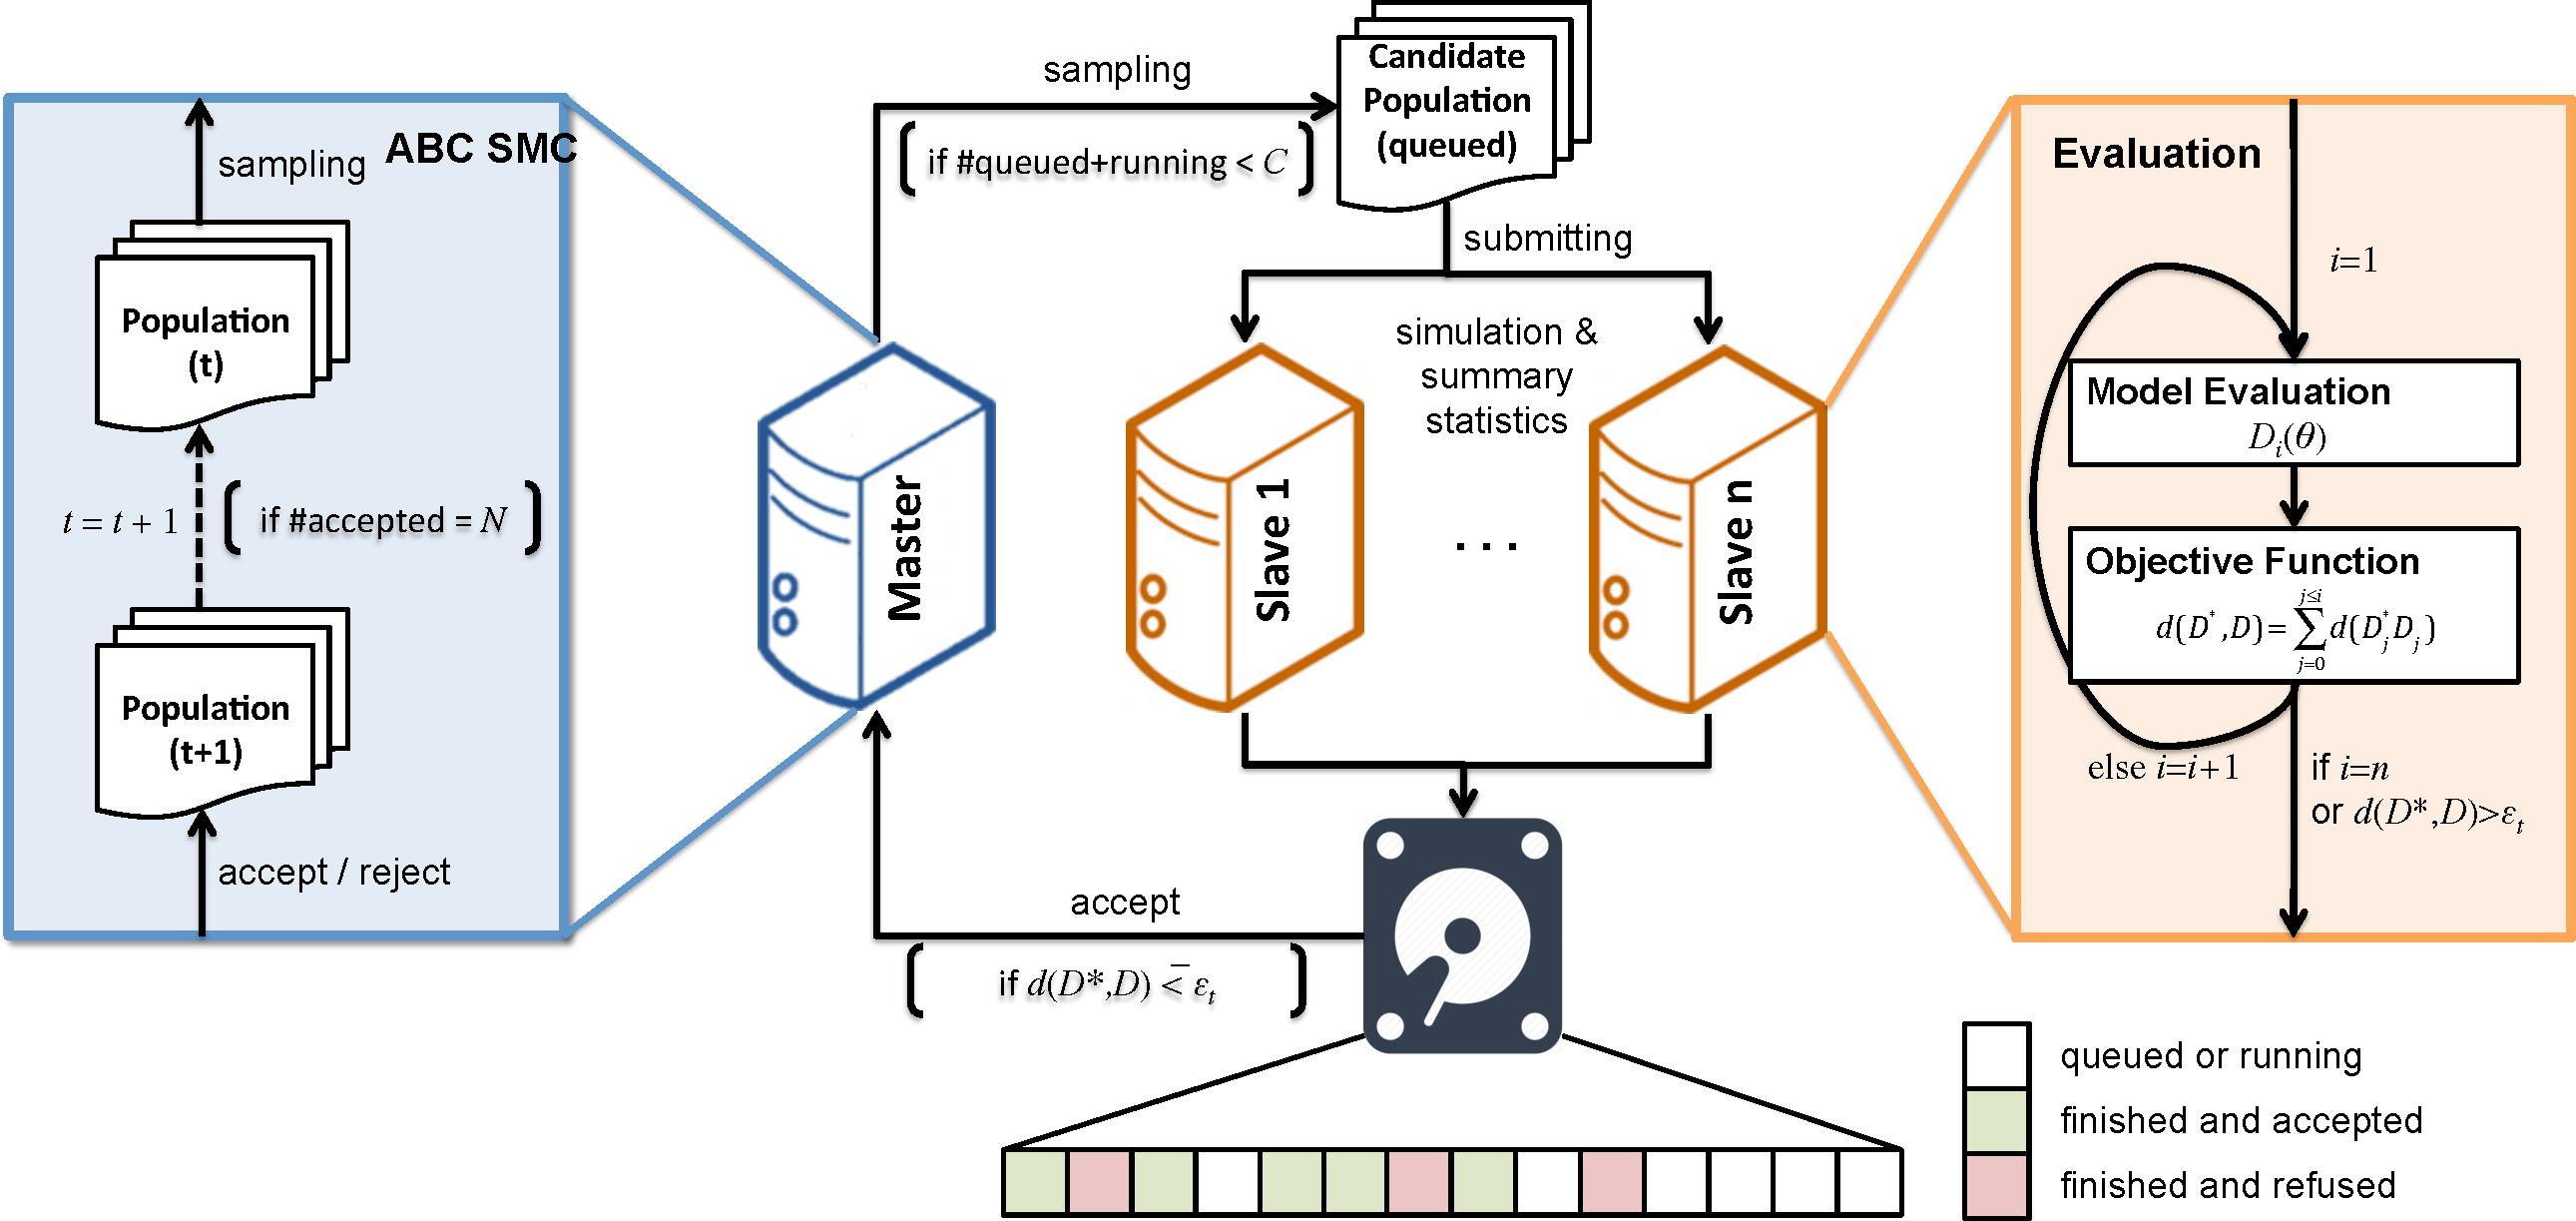
\includegraphics[width=\textwidth]{Figures/Pipeline.pdf}
\caption{{\bf Pipeline using cluster.}
The ABC method runs on a master machine. Each iteration $t$ new candidate parameters are drawn from a prior distribution and submitted to a queue. Slaves pick up candidates, simulate the model and calculate the summary statistics / distance to data. Then the master accepts those candidate with distances below a threshold $\epsilon$ and replaces all finished model evaluations with new samples on the queue.}
\label{fig1}
\end{figure}

Waiting for all jobs between the first $n_{pop}$ accepted ones to be finished is essential to avoid a bias towards parameters with faster model simulations. For the same reason all accepted jobs within the first consecutively finished which exceed the population size of $n_{pop}$ have to be ignored. 

\jh{can we design a simple example in which we see the bias which is introduced if we do not keep track of the order?}

\subsection*{Artificial data (2D)}

In order to assess the performance of ABC SMC we created a toy data set for a reference parameters $\hat{\theta}$ (see Material \& Methods). The model used to create the data is a tumor growth model which considers cell proliferation to be exclusively controlled by available space and extra-cellular matrix (ECM). Fig.~\ref{fig2} shows a sequence of simulation snapshots illustrating the model evolution over time and a respective experimental micrograph. The data consists of growth curves (spheroid radius) over time and histological data about cell proliferation and ECM extracted from the respective marker distributions, Ki67 and ColIV.  

In the following sections we present one inference run in detail and the results of a sensitivity analysis for different population sizes and additive (measurement) noise. 

\paragraph{Parameter Inference}


\begin{figure}[!h]
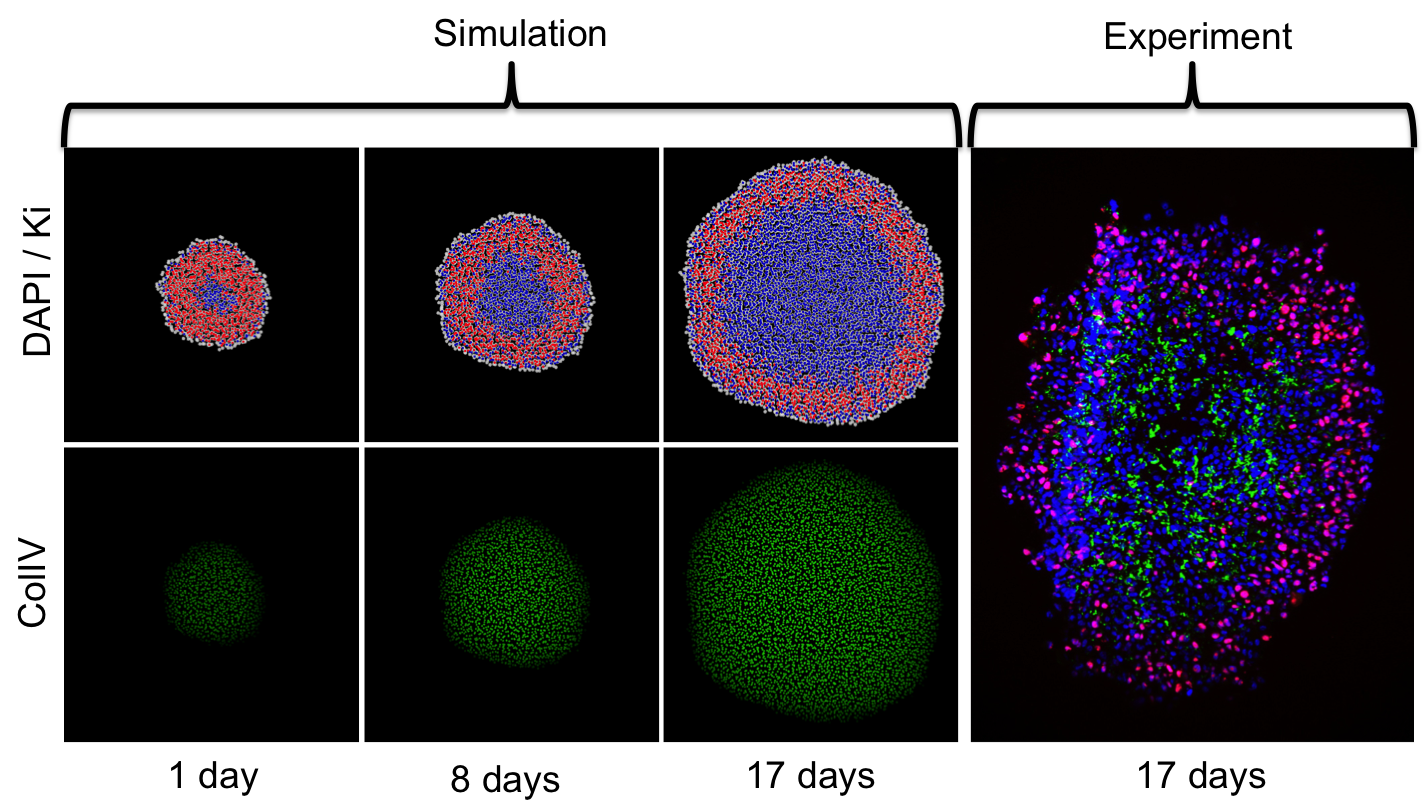
\includegraphics[width=\textwidth]{Figures/SimulationSnapshots}
\caption{{\bf Histological information in in-silicio and in-vitro data.}
The cross sections show cell stained with DAPI for cell nucleus (blue), Ki67 for proliferation (red), and ColIV  for extra-cellular matrix (green).}
\label{fig2}
\end{figure}


%\begin{figure}[h]
%\includegraphics[width=\textwidth]{Figures/FitToyData1.eps}
%\caption{{\bf Artificial data and fits for 5 (color-coded) generations (complete dataset).}
%Todo: add simulation snapshots and color legends.}
%\label{fig2}
%\end{figure}

Fig.~\ref{fig3} shows the comparison of data and model prediction of the parameter populations evolving over iterations.

For the inference of the model parameters used to create the artificial data all parameters can be identified. Nevertheless, the coupling parameter between cellular model and extracellular matrix, $e^{crit}$, needs a lot of evaluations and remains with a very large uncertainty. 

We also can observe that the acceptance rate of candidate samples becomes dramatically low for epsilon $<$ distance at the optimum itself.

\begin{figure}[htbp]
\begin{minipage}[t]{0.33\textwidth}
%\textbf{A} \hspace{180pt} \textbf{B} \\
\textbf{A}
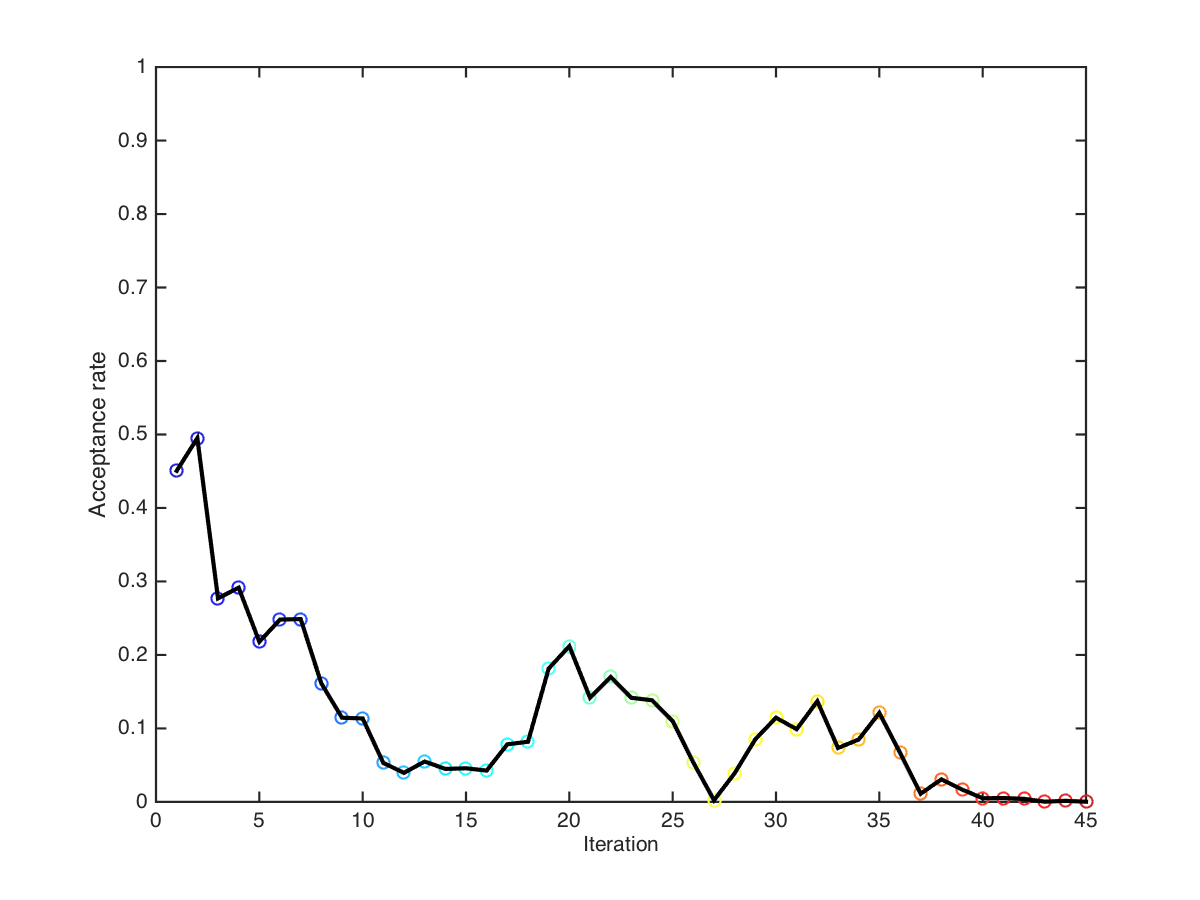
\includegraphics[width=\textwidth]{Data/TumorToyData2D_0.001merr_100pop_GCKI67ECM_NEW_acceptanceRate}\\
\textbf{B}
\includegraphics[width=\textwidth]{Data/TumorToyData2D_0.001merr_100pop_GCKI67ECM-objFunc}
\end{minipage}
\begin{minipage}[t]{0.66\textwidth}
\textbf{C}\\
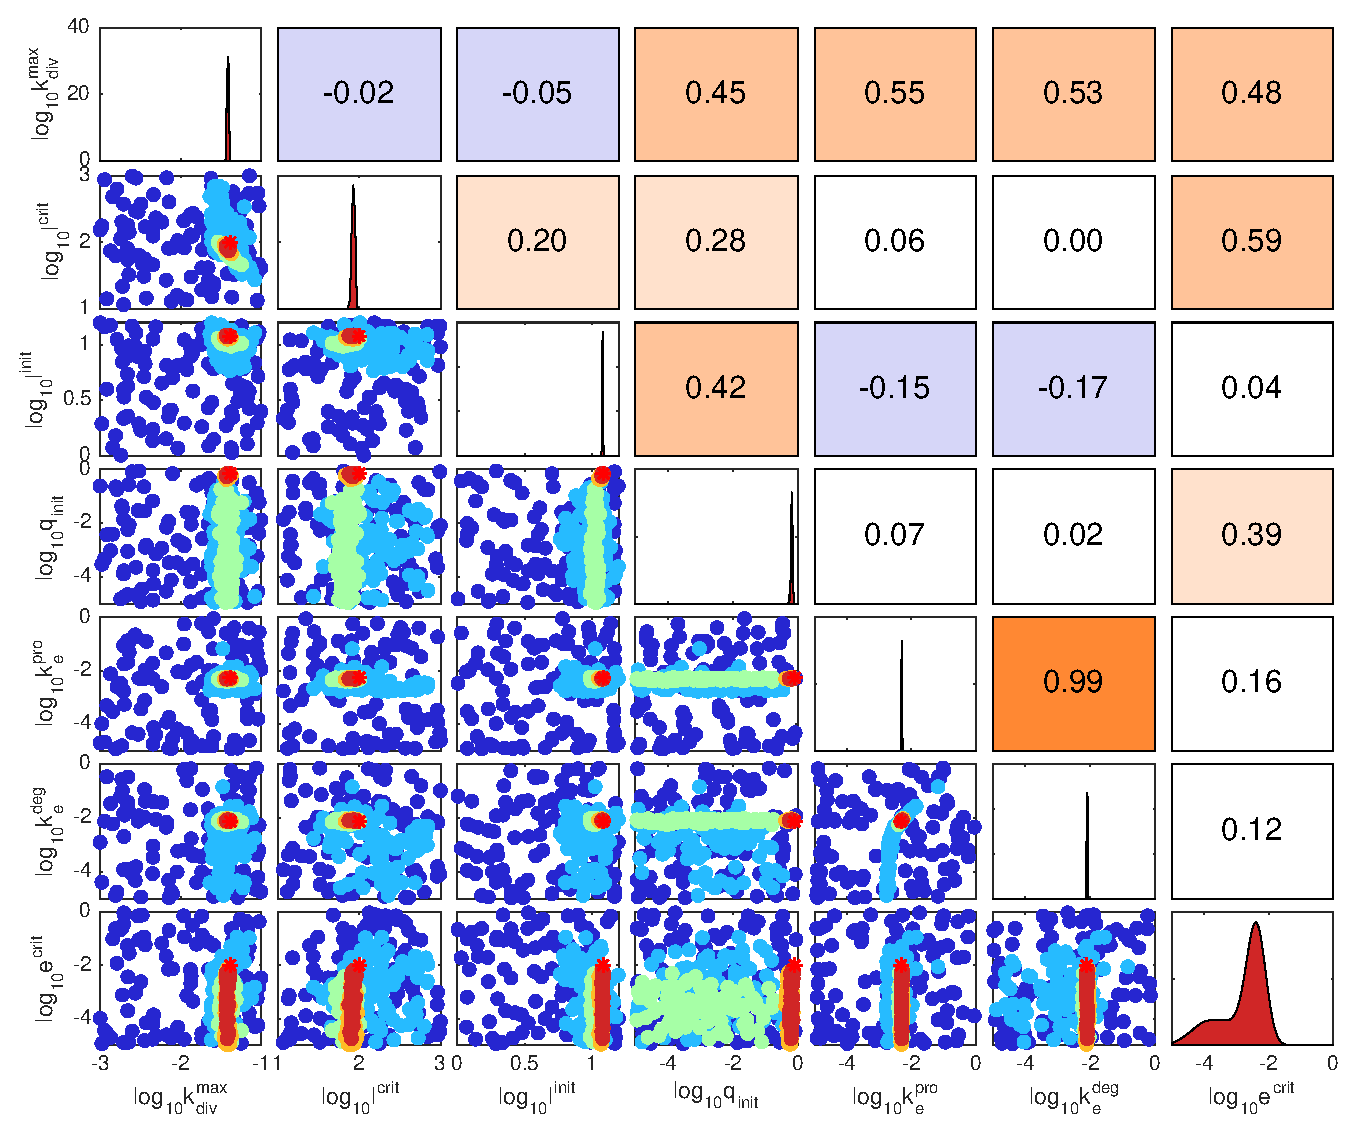
\includegraphics[width=\textwidth]{Data/TumorToyData2D_0.001merr_100pop_GCKI67ECM-scatterPlotMatrix}
\end{minipage}
\textbf{D}\\
\includegraphics[width=\textwidth]{Data/TumorToyData2D_0.001merr_100pop_GCKI67ECM-fits}
\caption{{\bf Artificial data and fits for 5 (color-coded) generation (complete dataset).}
\textbf{A}  acceptance rate over iteration; \textbf{B} $\epsilon$ threshold (cyan) and distance of the accepted population (blue) over iteration; for comparison the median distance at the optimum is depicted (red); \textbf{C} scatter matrix for 5 (color-coded) generation. todo: color spectrum. \textbf{D} Artificial data and fits for 5 (color-coded) generations (complete dataset).}
\label{fig3}
\end{figure}


%%%%%%
%%%%%%
\paragraph{Sensitivity to Population/Sample Size}
Fig.~\ref{fig4} illustrates that the population size has an critical impact on the convergence of the algorithm. If the population size is chosen too small, in our case 20, then convergence can not be assured. On the other hand we observe no significant improvement for an increase from 100 to 200. So for the means of limiting the cluster load per iteration all following parameter inference runs will be done with a population size of 100.

\begin{figure}[htbp]
\textbf{A} \hspace{180pt} \textbf{B} \\
\includegraphics[width=0.49\textwidth]{Data/TumorToyData2D_0.001merr_XXX0pop_GCKI67ECMfunctionEvaluations}
\includegraphics[width=0.49\textwidth]{Data/TumorToyData2D_0.001merr_XXX0pop_GCKI67ECMobjectiveFunction}\\
 \textbf{C} \\
\includegraphics[width=\textwidth]{Data/TumorToyData2D_0.001merr_XXX0pop_GCKI67ECMindependentBoxplots}\\
 \textbf{D} \\
\includegraphics[width=\textwidth]{Data/TumorToyData2D_0.001merr_XXX0pop_GCKI67ECMfit}\\
\caption{{\bf Sensitivity to Population/Sample Size.}
\textbf{A}  number of function evaluations over iteration; \textbf{B} threshold over iteration; \textbf{C} box plot of final sample for different population sizes. \textbf{D} final fits.}
\label{fig4}
\end{figure}


%%%%%%
%%%%%%
\subsection*{Experimental data (2D)}
Fig.~\ref{fig:exp2d} 

no histological info on proliferation (Ki67) leads to wrong predictions cellular kinetic param.
kinetic ECM param. not identifiable without hist. info. on ECM (ColV)


\begin{figure}[htbp]
\textbf{A}\\
%\includegraphics[width=0.49\textwidth]{Figures/FitToyData5a}
%\includegraphics[width=0.49\textwidth]{Figures/FitToyData5b}
\includegraphics[width=\textwidth]{Data/Tumor2dGCXXXindependentBoxplots}\\
\textbf{B}\\
%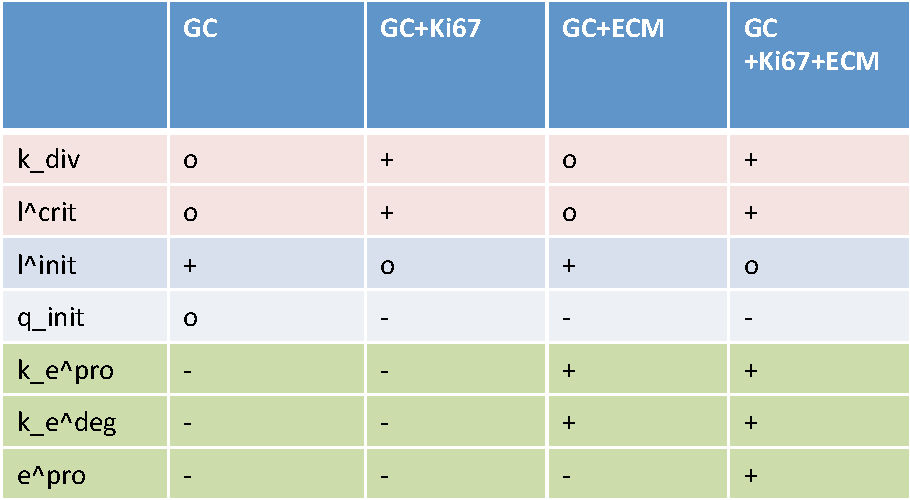
\includegraphics[width=\textwidth]{Figures/FitExpDataIdentifiabilityTable}\\
\begin{tabular}{r| r r r r }
& &KI67 &ECM &KI67ECM \\
\hline 
$k_{div}^{max}$&+ &+ &++ &+ \\
$l^{crit}$&+ &++ &+ &+ \\
$l^{init}$&++ &+ &+ &+ \\
$q_{init}$&++ &+ &+ &+ \\
$k_{e}^{pro}$&- - &- - &++ &+ \\
$k_{e}^{deg}$&- - &- - &++ &+ \\
$e^{crit}$&- - &- &- &++ \\
\end{tabular}

\begin{tabular}{r| r r r r }
& &KI67 &ECM &KI67ECM \\
\hline 
$k_{div}^{max}$& 0.815 & 0.660 & 1.000 & 0.509 \\
$l^{crit}$& 0.102 & 1.000 & 0.122 & 0.779 \\
$l^{init}$& 1.000 & 0.237 & 0.602 & 0.176 \\
$q_{init}$& 1.000 & 0.476 & 0.387 & 0.468 \\
$k_{e}^{pro}$& 0.014 & 0.019 & 1.000 & 0.260 \\
$k_{e}^{deg}$& 0.017 & 0.025 & 1.000 & 0.198 \\
$e^{crit}$& 0.046 & 0.063 & 0.081 & 1.000 \\
\end{tabular}

\textbf{C}\\
\includegraphics[width=\textwidth]{Data/Tumor2dGCXXXfit}
\caption{{\bf Different combinations of experimental data sets.}
\textbf{A} box plot for different combinations of data sets; \textbf{B} identifiablitity table (+ identifiable, o large uncertainty, - unidentifiable); \textbf{C} final fits and scenarios.}
\label{fig:exp2d}
\end{figure}

%%%%%%
%%%%%%
\subsection*{Experimental data (3D)}
Fig.~\ref{fig:exp3d} 

\begin{figure}[htbp]
\begin{minipage}[t]{0.33\textwidth}
%\textbf{A} \hspace{180pt} \textbf{B} \\
\textbf{A}
\includegraphics[width=\textwidth]{Data/Tumor3dGCKI67ECM-acceptanceRate.eps}\\
\textbf{B}
\includegraphics[width=\textwidth]{Data/Tumor3dGCKI67ECM-objFunc.eps}
\end{minipage}
\begin{minipage}[t]{0.66\textwidth}
\textbf{C}\\
\includegraphics[width=\textwidth]{Data/Tumor3dGCKI67ECM-scatterPlotMatrix.eps}
\end{minipage}
\textbf{D}\\
\includegraphics[width=\textwidth]{Data/Tumor3dGCKI67ECM-fits.eps}
\caption{{\bf Artificial data and fits for 5 (color-coded) generation (complete dataset).}
\textbf{A}  acceptance rate over iteration; \textbf{B} $\epsilon$ threshold (cyan) and distance of the accepted population (blue) over iteration; for comparison the median distance at the optimum is depicted (red); \textbf{C} scatter matrix for 5 (color-coded) generation. todo: color spectrum. \textbf{D} Artificial data and fits for 5 (color-coded) generations (complete dataset).}
\label{fig:exp3d}
\end{figure}

\begin{figure}[htbp]
\includegraphics[width=\textwidth]{Data/TumorXXXdGCKI67ECMindependentBoxplots}
\caption{{\bf Fitting experimental data: 2d versus 3d model.}
}
\label{fig:exp2dvs3d}
\end{figure}


%\begin{table}[!ht]
%\begin{adjustwidth}{-2.25in}{0in} % Comment out/remove adjustwidth environment if table fits in text column.
%\caption{
%{\bf Table caption Nulla mi mi, venenatis sed ipsum varius, volutpat euismod diam.}}
%\begin{tabular}{|l|l|l|l|l|l|l|l|}
%\hline
%\multicolumn{4}{|l|}{\bf Heading1} & \multicolumn{4}{|l|}{\bf Heading2}\\ \hline
%$cell1 row1$ & cell2 row 1 & cell3 row 1 & cell4 row 1 & cell5 row 1 & cell6 row 1 & cell7 row 1 & cell8 row 1\\ \hline
%$cell1 row2$ & cell2 row 2 & cell3 row 2 & cell4 row 2 & cell5 row 2 & cell6 row 2 & cell7 row 2 & cell8 row 2\\ \hline
%$cell1 row3$ & cell2 row 3 & cell3 row 3 & cell4 row 3 & cell5 row 3 & cell6 row 3 & cell7 row 3 & cell8 row 3\\ \hline
%\end{tabular}
%\begin{flushleft} Table notes Phasellus venenatis, tortor nec vestibulum mattis, massa tortor interdum felis, nec pellentesque metus tortor nec nisl. Ut ornare mauris tellus, vel dapibus arcu suscipit sed.
%\end{flushleft}
%\label{table1}
%\end{adjustwidth}
%\end{table}


%%%%%%
%%%%%%
%%%%%%
\section*{Discussion}


spatial moments


% You may title this section "Methods" or "Models". 
% "Models" is not a valid title for PLoS ONE authors. However, PLoS ONE
% authors may use "Analysis" 
\section*{Materials and Methods}
\subsection*{Model}
The test model we use is based on the spatial multi-scale model proposed by \cite{Jagiella2015} to describe in-vitro tumor growth. It is a hybrid approach of an individual-based model for tumor cells and a system of partial differential equations describing the molecular kinetics of extra-cellular matrix (ECM), the key metabolites and waste material from cellular debris of necrotic cells. 

\paragraph{Cell model:} Cells populate a static unstructured lattice (max. 1 cell per lattice site). They can be either \emph{alive} or \emph{necrotic}. Cells can perform a birth and death process, if they are alive, or a lysis process, if they are necrotic. The respective transition rates are defined by the following equations:
\begin{align}
	k_{div}  &= {\color{red}{k_{div}^{max}}} H(e-{\color{red}{e^{crit}}}) H(k^{a}_{pro}) e^{-l/{\color{red}{l^{crit}}}},\\
	k_{nec} &= {\color{red}{k_{nec}^{max}}} H(k^{a}_{pro}),\\
	k_{lys} &= const.
\end{align}
and depend on the local molecular concentrations of ECM ($e$), oxygen ($o$), waste ($w$) and the production rate of ATP ($k^{a}_{pro}$). The division rate further depends on the distance $l$ a cell would have to push surrounding cells away toward the closest free lattice site in order to free space for the second daughter cell.

\begin{table}[!ht]
\begin{adjustwidth}{-0in}{0in} % Comment out/remove adjustwidth environment if table fits in text column.
\caption{
{\bf Model parameters.}}
\begin{tabular}{|l|r|r|r|r|r|}
\hline
{\bf Parameter} &{\bf Symbol} &{\bf Unit}  &{\bf Value} &{\bf Range (Setting I)} &{\bf Range (Setting II)}\\ \hline
division rate &$k_{div}^{max}$\\ \hline
necrosis rate &$k_{nec}^{max}$\\ \hline
lysis rate &$k_{lys}$\\ \hline
\end{tabular}
\begin{flushleft} The table shows all model parameters with there respective values. For the different parameter inference settings the ranges for those parameters which were .
\end{flushleft}
\label{table1}
\end{adjustwidth}
\end{table}


\paragraph{Molecular model:} The molecular dynamics is described by system of partial differential equations as follows:
\begin{align}
	\partial_{t} e &= {\color{red}{k^{e}_{pro}}} c - {\color{red}{k^{e}_{deg}}} e,\\
	\partial_{t} g &= D \nabla g - k^{g}_{con} c,\\
	\partial_{t} o &= D \nabla o - k^{o}_{con} c,\\
	\partial_{t} a &=k^{a}_{pro}c - k^{a}_{con} c, k^{a}_{pro} =  2k^{g}_{con} c + 17/3 k^{o}_{con},\\
	\partial_{t} w &= {\color{red}{k^{w}_{pro}}} c_{nec} - {\color{red}{k^{w}_{deg}}} w,\\
\end{align}
where $c=1$, if the a living cell is occupying the volume, or $c_{nec}=1$, if a necrotic cell is occupying the same volume. Else $c=c_{nec}=0$.

\paragraph{Initial \& boundary conditions:}
The initial cell population occupies all lattice sites within a sphere of radius {\color{red}{$l^{init}$}}. A fraction of those cells $\color{red}{q_{init}}$ is quiescent, while the rest enters the cell cycle.

\paragraph{Parameters:} 

The resulting model is stochastic and only numerically solvable. Here we use the Gillespie algorithm to simulate a possible evolution of the cell population and solve the stead state problem for the molecular system after each update. The parameters that are subject to optimisation are indicated in red.

\subsection*{Data} 
We used two types of data: the growth curves of multi-cellular spheroids over time and histological information on the spatial distribution of proliferating cells and extra-cellular matrix at a certain moment of the experiment.

\subsection*{ABC}
The ABC SMC method used in this paper is based on Toni et al. \cite{Toni2009}. The idea can be briefly summarised as the following: 

\begin{itemize}
\item[S1)] initialize: $t=1, p_{1}(\theta) = \pi(\theta)$, $\epsilon_{1} = \infty$
\item[S2.0)] set $i = 1$ \emph{\#new generation }
\item[S2.1)] draw $\theta_{t}^{i}$ from proposal distribution $p_{t}$ \emph{\#sample}
\item[S2.2)] draw $y_{t}^{i} = f(\hat{x}, \theta_{t}^{i})$ \emph{\#simulate}
\item[S2.3)] if $d( y_{t}^{i}, \hat{y}) \ge \epsilon_t$ go to S2.1. \emph{\#reject}
\item[S2.4)] if $i = n$ set $t=t+1$ and go to S2.0.  \emph{\#next generation}
\end{itemize}

Each iteration $t \ge 1$ we sample candidate parameter vectors $\theta^*$ from a prior distribution $p^{(t)}(\theta)$ and evaluate the model $y^{*} = f(x, \theta^*)$. If the corresponding  objective function value is $\delta(y^{*}, y) < \varepsilon^{(t)}$, then $\theta^*$ will be accepted and added to $\Theta^{(t)}$. If a minimal number of $n$ accepted parameter vectors is reached, then the algorithm will proceed to the next iteration, $t = t+1$. The main extension of ABC SMC compared to ABC is to itertively adapt both, the prior distribution $p^{(t)}(\theta)$ and the acceptance threshold $\varepsilon^{(t)}$.

\paragraph{Choice of Prior Distribution $p^{(t)}(\theta)$}
Here we chose a Gaussian perturbation kernel:
\begin{equation}
	p^{(t)}(\theta) = \sum_{i}\frac{1}{w^{(t)}_{i}} (2\pi)^{-k/2} |\Sigma|^{-1/2}e^{-1/2(x-\mu)^{T}\Sigma^{-1}(x-\mu)},
\end{equation}
where $\mu$ is the mean and $\Sigma$ is the standard deviation of the current population $t$.
\paragraph{Choice of $\varepsilon$-thresholds} The threshold distance $\epsilon$ for accepting a candidate parameter is chosen to be the median among the actual population 
\begin{equation}
	\epsilon^{(t)} = \text{median} \{ \theta^{(t)} \}
\end{equation}


\paragraph{(Surrogate Approximation)}





%%%%%%
%%%%%%
%%%%%%
\section*{Supporting Information}

% Include only the SI item label in the subsection heading. Use the \nameref{label} command to cite SI items in the text.
%\subsection*{S1 Video}
%\label{S1_Video}
%{\bf Bold the first sentence.}  Maecenas convallis mauris sit amet sem ultrices gravida. Etiam eget sapien nibh. Sed ac ipsum eget enim egestas ullamcorper nec euismod ligula. Curabitur fringilla pulvinar lectus consectetur pellentesque.
%
%\subsection*{S1 Text}
%\label{S1_Text}
%{\bf Lorem Ipsum.} Maecenas convallis mauris sit amet sem ultrices gravida. Etiam eget sapien nibh. Sed ac ipsum eget enim egestas ullamcorper nec euismod ligula. Curabitur fringilla pulvinar lectus consectetur pellentesque.
%
%\subsection*{S1 Fig}
%\label{S1_Fig}
%{\bf Lorem Ipsum.} Maecenas convallis mauris sit amet sem ultrices gravida. Etiam eget sapien nibh. Sed ac ipsum eget enim egestas ullamcorper nec euismod ligula. Curabitur fringilla pulvinar lectus consectetur pellentesque.
%
%\subsection*{S2 Fig}
%\label{S2_Fig}
%{\bf Lorem Ipsum.} Maecenas convallis mauris sit amet sem ultrices gravida. Etiam eget sapien nibh. Sed ac ipsum eget enim egestas ullamcorper nec euismod ligula. Curabitur fringilla pulvinar lectus consectetur pellentesque.
%
%\subsection*{S1 Table}
%\label{S1_Table}
%{\bf Lorem Ipsum.} Maecenas convallis mauris sit amet sem ultrices gravida. Etiam eget sapien nibh. Sed ac ipsum eget enim egestas ullamcorper nec euismod ligula. Curabitur fringilla pulvinar lectus consectetur pellentesque.

%%%%%%
%%%%%%
%%%%%%
\section*{Acknowledgements}

%(this will go in the funding statement provided in the online submission system)

This work was supported by the Postdoctoral Fellowship Program (PFP) of the Helmholtz Zentrum M\"unchen (J.H.).

%%%%%%
%%%%%%
%%%%%%
\section*{Author Contributions}

Conceived and Designed the Methods: NJ DR FJT JH.
Developed Models: NJ.
Performed Numerical Experiments: NJ DR.
Wrote the Paper: NJ FJT JH.

\nolinenumbers

%%%%%%
%%%%%%
%%%%%%
\bibliographystyle{plos2015}
\bibliography{Database,bibliography}


\end{document}

